\begin{savequote}
`` ... omnium rerum simulatio vitiosa est (tollit enim iudicium veri idque adulterat) ... delet enim veritatem''
\qauthor{Marcus Tullius Cicero, \emph{Laelius De Amicitia}, 44 BC}
\end{savequote}




\chapter{Conclusions and Future Work}
%\minitoc

In this chapter we present a synopsis of the thesis work and give an outline of
further work to be done.

\section{Code Testing and Code Comparison}
A new MHD code was modified to include the effects of radiative cooling and to
be able to simulate binary jets from orbiting sources in three dimensions
(see Chapter 2).
The code was comprehensively tested using both experimental results and standard
tests from the literature.
The tests included both purely hydrodynamical results in one and two dimensions
and magnetohydrodynamical problems.
A simulation of the Orszag-Tang vortex was compared with published results to
test the ability of the code to maintain divergence of magnetical field equal to
zero.
Furthermore, a code comparison was performed  to establish the veracity of our results for problems relevant to astrophysical jets. 


\section{Jets from Binary Protostars}
The propagation and evolution of binary jets was studied for a range of
conditions (see Chapter 3).
Previous work on simulations of jets from young stars (see Chapter 1 for a
summary) have mainly been focused on single jets, although a significant
proportion of stars are binaries. 
The frequency of binary jets is low compared to the frequency of single
jets observed from protostars.
In Chapter 3 we examined the effect of having a source in orbital motion using a
numerical simulation.
The orbiting jets have to do extra work moving the ambient medium in a
transverse direction, which has the effect of a transverse wind shredding the
jet.
We found that while orbital motion could contribute to a twisted morphology and
eventual breakup, the source motion required exceeds the observed values (e.g. for the
case of the young binary LDN1551 IRS 5) by an order of magnitude.

The lateral expansion of a jet can have a significant effects for a young binary
jet. If the sources are close together, as in a close
binary, the bow shock of one jet can distort the beam of the secondary jet. 
For the hydrodynamic case, it was shown that jets from LDN1551 IRS 5 interact strongly due to thermal pressure of the fast jet's bow shock upon the beam of the slow jet.
In order to compare this result against observations, the fraction of ionized
hydrogen in each cell was tracked during the simulation and the [SII] line
emission was calculated. A peak in the emission where the bow shock strikes the
beam was found. This is at approximately the same location as a bright ``knot''
seen in the HST [SII] images.

To study the effect of the magnetic field on the jet interaction a toroidal
magnetical field was introduced.
Observations of a high degree of polarization in LDN1551 at optical, infrared
and submillimetre wavelengths imply an ambient magnetic field is
present.
It is shown that the effect of the toroidal field is to exert a hoop stress on the jet pair and thus force together the diverging pair of jets.
This effect is seen in the observations of LDN1551 IRS 5 where the jets
initially diverge but then turn to pursue a roughly parallel course.

In summary, the results of this section show that orbital motion has little
effect on the stability and lifetime of a binary jet. However when two jets are
present, a faster one can dominate its slower companion and this can account for
the paucity of binary jets in the observations. The presence of a magnetic field
in the observed configuration can provide further redirection and enhance the
interaction of the two jets until they appear to almost merge.

\section{Jets in Evacuated Ambient Media}
The propagation in jets in partially evacuated ambient media was studied (see
Chapter 5).
The aim of the Chapter was to show that the prehistory of the outflows and jets from the same source affects the current outflow.
A secondary aim was to show the effects of a jet on the circulation model.
 Although much previous work on jet propagation has been done, many studies assume that
 the jet is the first to propagate into its environment without assuming any
 prehistory of jets. In addition many studies assume a uniform density and
 pressure without lateral variation. 
 This assumption is removed in the present work, which models a jet entering a cavity. We study the effects of the cavity on jets of
 different densities, with and without pulsing and cooling and try an identify
 the effect of such a cavity on observable quantities such as the speed, the aspect ratio and the
 morphology. 
A range of simulations were performed in both axisymmetry and 3D.
The effects of varying the presence of cooling, velocity variation in the input,
and different jet-to-ambient density ratios for cavities of different sizes were examined.
The density function of the cavity was parametrised in order to provide a measurable quantity.
This thesis shows three major effects of the evacuated cavity on the collimated jet.
\begin{itemize}
\item Recollimation. Using the aspect ratio to measure the amount of collimation,
we find consistently large increases up to 140\% for one case. This results
clearly shows that the prehistory and ambient environment can have a large
effect on the recollimation of a jet as it propagates outward from the source.
\item Acceleration. In all cases where a cavity is present, advance speeds are
increased, consistent with analytical predictions from one-dimensional ram pressure balances.
\item An overall decrease in the amount of structures associated with
instabilities in the cocoon is seen. 
Linear theory implies the growth rate for the Kelvin-Helmholtz instability is
inversely proportional to the Mach number,  
so this results is consistent with the increased Mach number of the accelerated,
recollimated jets.
number of the jet.
\end{itemize}
The hydrodynamic pressure exerted by the walls of the cavity compresses and focuses the cocoon in all cases. 
The centre of the cavity also has much less material to resist the incoming shock and there is a resulting acceleration in the jet.
The combination of compression and acceleration greatly reduces the amount of cooling instabilities. 
Signs of jets entering cavities such as these may be used to identify examples of circulation flow in observations.



%\section{Part III}
%The aim of the third part of this thesis was to map the extinction of the entire galactic plane.  To this end, a code was written to generate relative extinction maps from 2MASS star catalogue data.  Using the code, relative extinction of the entire galactic plane was estimated at an unprecedented resolution.  Galactic extinction maps and star density maps were created.  From the large scale star density maps, new clusters can be identified, while from the extinction maps, observers can obtain more accurate values of the opacity index. To this end, the data and code have both been made available over the Internet to the scientific community.  


\pagebreak

\section{Future Work}

%The problem of binary jets and binary star formation is still important and there are several future research opportunities in this topic.
%Higher resolution is still important and will be possible within the next few years.

\subsection{Jets from Binary Protostars}
%In Chapter 4 we explored the propagation of binary jets and their interaction.
The propagation and interaction of jets is a very broad area and contains
several practical future research directions.
There are still several outstanding problems with binary jets from young stars.
An important question is whether the results based on observed quantities of
LDN1551 IRS 5 can be generalised.
A major requirement for further progress in direct simulation is a larger number
of observational samples of binary jets.  The number of observations remains low
- approximately 10 sources.  An observational search for binary jets in star
forming regions would be able to add extra constraints to the model.  In
particular, a better constraint on the geometry of the magnetic field, which may
be obtained using polarimetry, is desirable.  
While the best resolution
available was used in this thesis along with modern adaptive grid techniques,
resolution is still relatively low in three dimensions.  A higher resolution
study would give a more accurate quantitative estimate of the emission from the
interaction region.  Furthermore, in order to compare results with observations
properly, it would be desirable to include a chemical network in the code, so
emission maps for additional species, such as CO, could be produced.  A future
study could include the effects of precession as well as orbital motion.
Precessing jets will have enhanced interaction and are likely to show increased
dynamical instability.

Another open question concerns the production of X-rays from binary jets.  As
discussed in Chapter 4, the generation of X-rays from shocks in the case of
L1551 IRS 5 requires velocities which are greater than those inferred
from observations at other wavelengths.  Imagining the binary jet system as a
pair of mutually orbiting flux tubes, the probability of reconnection events
occurring immediately springs to mind.  For a physically meaningful study of
reconnection processes within the binary jet, use of non-ideal MHD techniques such
as e.g. Hall-MHD would be desirable.  Some progress, however can be made
studying using resistive MHD.  As a preliminary step towards this, we have
modelled 3D reconnection processes in a current sheet, over a range of
perturbation modes.  The purpose of the study is to constrain the large amount
of thermal energy released in the reconnection process.  
For wave modes with $k> 1/a$, where $k$ is the wave number and $a$ is the current sheet thickness, along
with the release of thermal energy, we
observe in early simulations the formation of magnetic islands on the current sheet, which are
usually associated with the tearing mode instability. Encouragingly, the
critical value is in agreement with that found through the MHD analysis in the linear regime by \citet{furth2004fri}.
Three-dimensional studies of the nonlinear regime are ongoing.

%In this general three-dimensional study, the role of the tearing mode
%instability in the growth and sustenance of supersonic turbulence in
%star-forming regions

%Extension to binary AGN jets, recent results 
%Supermassive binary black hole mergers.
%Grenoble.

\subsection{Jets in Evacuated Cavities}

The evacuated cavity model for jet recollimation can be further enhanced by
including a treatment of the magnetocentrifugal wind launching mechanism.
%Higher resolution three-dimensional simulations for more realistic cavities.
%In addition a greater parameter space could be explored with the inclusion of more 3D effects such as precession, turbulent gas and magnetic field.
This is a non-trivial problem, and necessitates the inclusion of gravity and
magnetic field.
An internal boundary is necessary around the gravitational source to prevent
numerical difficulties when the radius approaches zero.
Non-ideal effects such as resistivity are needed to allow accreting matter to slip through the magnetic
field lines and gravitate towards the central object. 
Cooling is required within the disk to compensate for the effect of Joule
heating, which tends to puff up the disk.
\citet{2007astro.ph..3064Z} give a comprehensive treatment of the subject.
We have performed such a simulation in order to calculate the size of the cavity
generated by such a wind.
We have also increased the domain of the simulation to study the long term
evolution of the MHD wind model, examine the effects of boundary conditions on
the jet collimation, and compare against observations of rotation in star
formation jets. This required the use of a stretched grid in
order to keep the simulation down to a manageable amount of computational time
and data. 
The simulation also requires a greatly increased number of timesteps (an order of magnitude
greater then in previous work), due to the much larger Keplerian rotation
period in the outer edges of the disk.
In Figure \ref{fig:MHDDiskWind} a plot of the large-scale MHD disk wind simulation is shown.
The bow shock, collimated disk wind and the disk itself are all present.
The cavity formed may be clearly seen to the left of the image.
It expands initially but then is recollimated along with the rest of the jet
near to the bow shock.
The simulation is still dynamically evolving and has not reached a
quasi-stationary state yet.
An important further study is to compare the results of the simulation to measurements of the jet rotation using Doppler
gradients.

Another important application of this model is
outside the star formation regime, for 
microquasars and AGN jets.
In the two-flow scenario, a classical MHD wind of the type 
shown in Figure \ref{fig:MHDDiskWind} confines a highly relativistic electron-positron
pair plasma beam \citep{1991ApJ...383L...7H}.
The MHD outflow plays a dual role in the model. It provides a cavity in which the electron-positron
beam can propagate. The outflow also prevents catastrophic Compton cooling from decelerating the
electron-positron beam by reheating it through second-order Fermi mechanism
thus allowing it to reach velocities approaching light speed 
\citep[typically 92-99\%,][]{1998MNRAS.300.1047R}. 
This acceleration mechanism can explain the apparently superluminal motions near
black-hole X-ray binaries observed by \citet{1992Natur.358..215M}. See \citet{1999ARA&A..37..409M} for a
review of observations of galactic superluminal sources.
The goal of this study is investigate the feedback between
the two flows, in particular the effect of a strongly heated and episodic set of
outburst on a collimating MHD wind. 
The MHD model is used to calculate the mean magnetic field and the radius of the
inner cavity as a function of height.
These constraints are then used to calculate the particle density and thermal
energy of the plasma inside the cavity using a relativistic particle code
\citep{2006A&A...454L...1S}.
An internally consistent model for ejections from black-hole X-ray binaries will
then be obtained.

%hich may explain the episodic outbursts seen in observations such as GR 1915+105.



\begin{figure}[t]
\centering
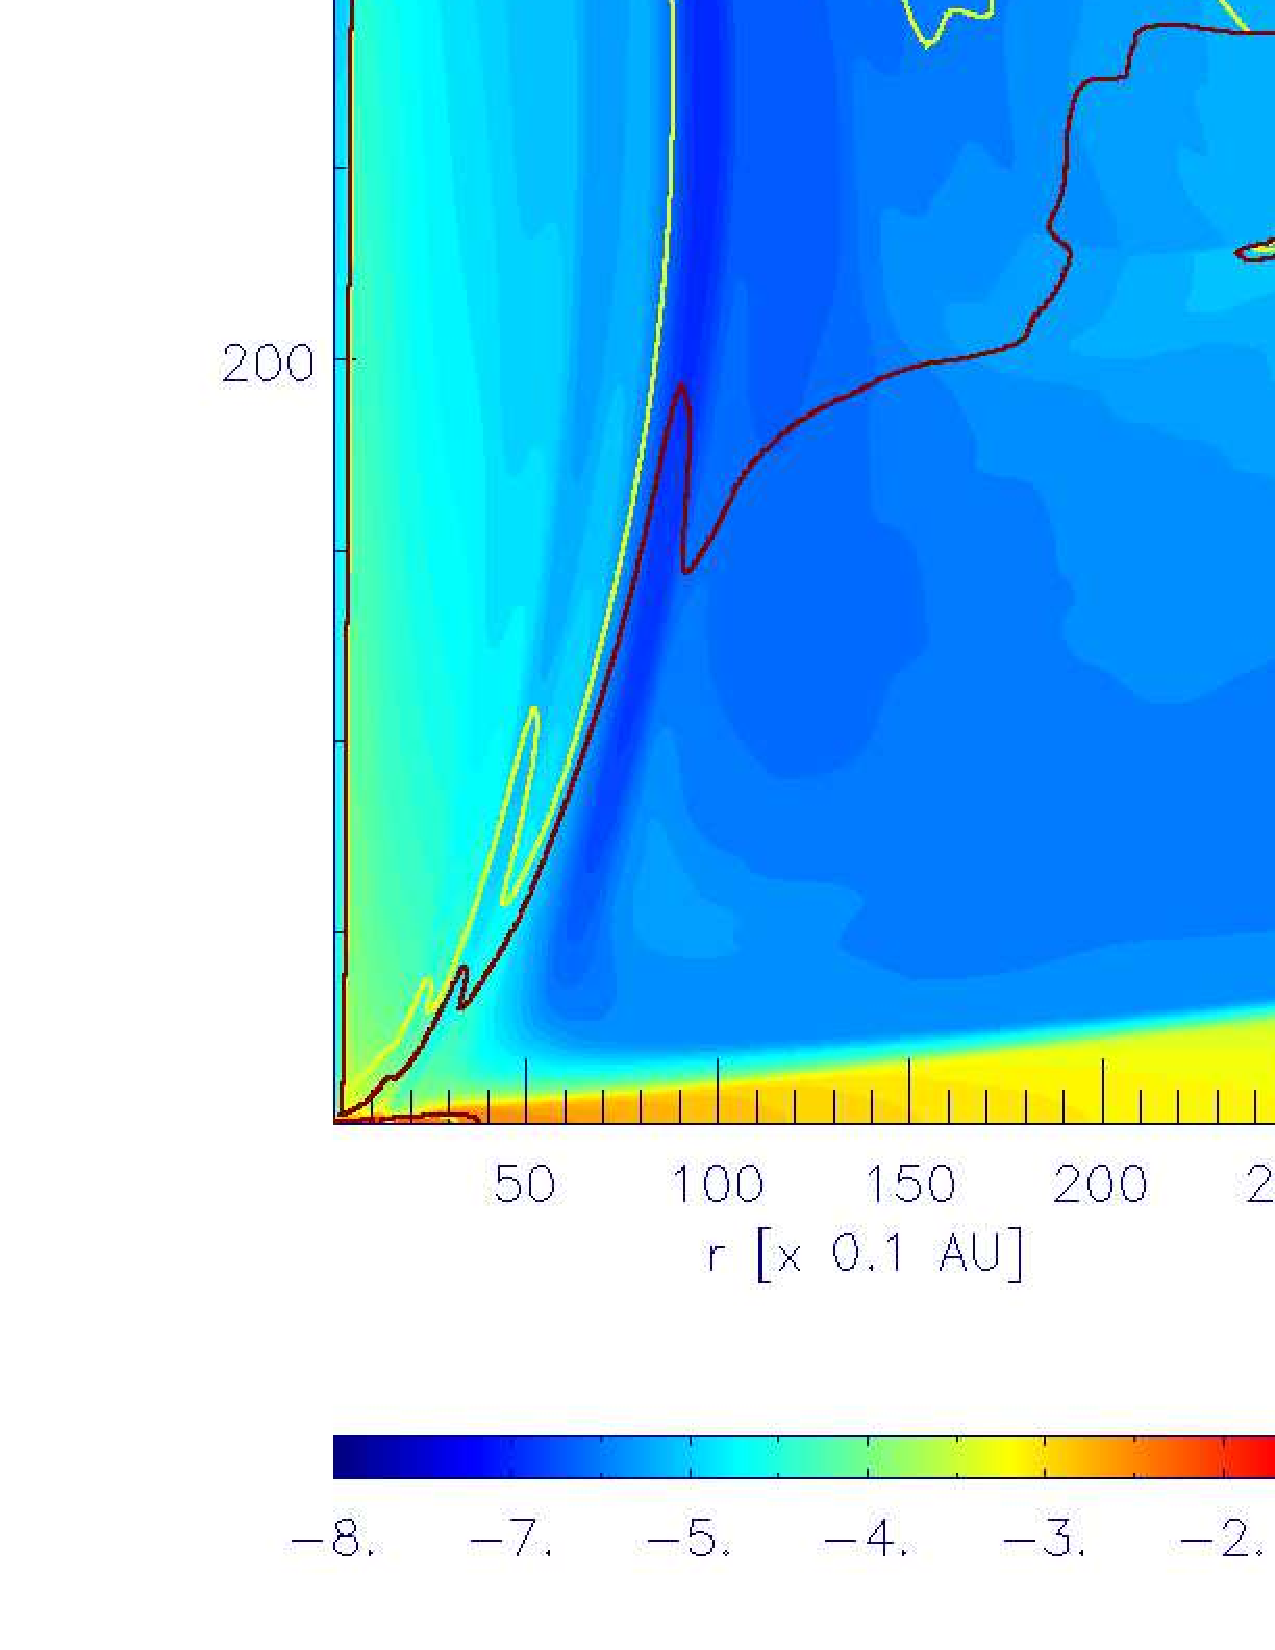
\includegraphics[height=21cm]{finalthes}
\caption{
Log density colourmap of axially symmetric MHD disk wind simulation at t=63.
(Time units are Keplerian periods a the disk inner radius)
As the disk wind moves upward from the disk it becomes collimated.
The fast magnetosonic and Alfv\'en surfaces are plotted as yellow and black
contours respectively.
}
\label{fig:MHDDiskWind} % label
\end{figure}



%\subsection{Galactic Plane Extinction Maps}


%The current model has calculated the colour excesses for use in the \citet{1994ApJ...429..694L} Near-Infrared Colour Excess method to determine an even better and less noisy extinction map. Ideally this more accurate method could be used for the whole sky in the next phase of this study.


